% Fichier généré automatiquement par tools/generate_corrections.py.
% Source : DYN/DYN-05-Methode/01_T/01_T.tex
% Statut : complété (2/2 question(s)).
\begin{corrigebox}[Corrigé complété]
\CorrigeQuestion{1}
\CorrigeSource{Réponse reprise d'un exercice homonyme de la banque ; la provenance exacte est indiquée dans le commentaire du fichier.}
% Réponse reprise de : STAT/STAT-03-Demarche/01_T/01_T.tex
\begin{marginfigure}
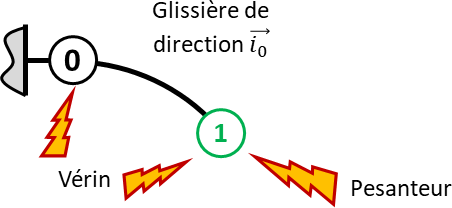
\includegraphics[width=.35\linewidth]{../../../STAT/STAT-03-Demarche/01_T/images/01_T_01_c}
\end{marginfigure}
\CorrigeQuestion{2}
On choisit les inconnues et les conventions positives de la figure,
        on écrit les relations de conservation/fermeture adaptées, puis on résout le
        système obtenu. Le résultat symbolique doit être homogène et vérifié dans les cas
        limites (entrée nulle, rapport unitaire ou position de référence).
\end{corrigebox}
